%% Supplementary Information — CILP
\documentclass[11pt,a4paper]{article}
\usepackage[margin=2.0cm]{geometry}
\usepackage{times}
\usepackage{mathtools,amssymb}
\usepackage{booktabs,longtable}
\usepackage{graphicx}
\usepackage[hidelinks]{hyperref}
\usepackage{natbib}
\usepackage{enumitem}
\usepackage{algorithm,algpseudocode}
\usepackage{setspace}
\usepackage{tabularx}
\usepackage{url}
\urlstyle{tt}
\setstretch{1.08}
\providecommand{\path}[1]{\url{#1}}

\title{Supplementary Information\\[0.3em]
\large Learning which edges to remove under a budget:\\
Counterfactual inverse link prediction for utility-preserving\\
social-network sparsification}
% Authors: finalize list before submission.
\author{}
\date{}

\begin{document}
\maketitle
\tableofcontents
\newpage

\section{S1 Dataset acquisition and preprocessing}
SNAP (LastFM, GitHub) and MUSAE (Facebook) public releases~\citep{rozemberczki2021multi}.
Symmetrization; self-loop and duplicate undirected-edge removal; multi-hot bag-of-words features.

\section{S2 Dataset audit and statistics}
\begin{center}\scriptsize
\begin{tabular}{@{}lrrr@{}}
\toprule
Statistic & LastFM & Facebook & GitHub \\
\midrule
Nodes & 7624 & 22470 & 37700 \\
Raw edge records & 55612 & 341646 & 578006 \\
Unique undirected edges & 27806 & 170823 & 289003 \\
Self-loops in tensor & 0 & 0 & 0 \\
Average degree & 7.294 & 15.205 & 15.332 \\
Median degree & 4.0 & 7.0 & 6.0 \\
Maximum degree & 216 & 709 & 9458 \\
Connected components & 1 & 1 & 1 \\
Giant-component ratio & 1.000 & 1.000 & 1.000 \\
Avg.\ clustering & 0.219 & 0.360 & 0.168 \\
Classes & 18 & 4 & 2 \\
Minority-class proportion & 0.0021 & 0.1481 & 0.2583 \\
Feature dimension & 7842 & 4714 & 4005 \\
Feature density & 0.0504 & 0.0030 & 0.0046 \\
Label homophily & 0.874 & 0.885 & 0.845 \\
Graph density & 9.57e-04 & 6.77e-04 & 4.07e-04 \\
\bottomrule
\end{tabular}
\end{center}

Processed graphs contain no self-loops.
Directed tensor encodings store both directions of each undirected edge; the unique undirected count is the scientific edge set used for budgets.

\section{S3 Train/development/test splits}
Seeds $0$--$9$; stratified $60/20/20$ train/development/test; masks under \texttt{data/splits/}.
The middle partition is termed the development set throughout.

\section{S4 Leakage audit}
\begin{center}\small
\begin{tabular}{@{}p{2.4cm}p{2.2cm}p{2.2cm}p{2.2cm}p{3.4cm}@{}}
\toprule
Stage & Train & Dev & Test & Permitted use \\
\midrule
Features & Yes & Yes & Yes & Shared $X$; no label-dependent featurization \\
Splits & Yes & Yes & Yes & Stratify masks only \\
Teacher $\Delta_{\mathrm{task}}$ & Yes & Yes (TD mask) & No & CE on train$\cup$development \\
Scorer fit & Yes & Used in grid & No & Fixed epoch loops in reported grid \\
Teacher size $n$ & --- & Yes (Facebook) & No & Select on development Macro-F1 @50\% \\
Final eval & --- & --- & Yes & After configuration is fixed \\
\bottomrule
\end{tabular}
\end{center}
\noindent\textit{Note.}
The middle partition is a development set, not an independent validation hold-out: it participates in teacher-target construction and Facebook teacher-size selection.
This is not test leakage, but the protocol is not fully validation-isolated.
A stricter design would construct teacher targets from training labels only and reserve development exclusively for configuration selection.

\section{S5 Counterfactual teacher}
CILP uses a composite multi-criteria teacher that combines deletion-induced effects with structural proxies.
\texttt{ExactCounterfactualTeacher.score\_edges} samples $n$ edges and returns $y^{\mathrm{cf}}$ plus component vectors.
The task-only teacher uses only the classification-loss component under the same encoder and concatenation fusion.

\section{S6 Exact deletion-importance criteria}

\paragraph{Task loss (deletion-induced).}
With frozen encoder/classifier,
$\Delta_{\mathrm{task}}=\mathrm{CE}_{TD}(G_{-e})-\mathrm{CE}_{TD}(G)$ on train$\cup$development nodes.

\paragraph{Connectivity change (deletion-induced).}
\[
\Delta_{\mathrm{conn}}(e{=}\{u,v\})
=\mathbf{1}[e\textrm{ is a bridge}]
+(\#\mathrm{comp}(G_{-e})-\#\mathrm{comp}(G))
+\max(0,\mathrm{giant}(G)-\mathrm{giant}(G_{-e}))/|V|.
\]

\paragraph{Representation shift (deletion-induced).}
$\Delta_{\mathrm{repr}}(e)=\mathrm{mean}_i\|h_i(G)-h_i(G_{-e})\|_2$.

\paragraph{Group impact (deletion-induced).}
$\Delta_{\mathrm{group}}(e)=\max(0, F1^{\mathrm{worst}}_{\mathrm{dev}}(G)-F1^{\mathrm{worst}}_{\mathrm{dev}}(G_{-e}))$.

\paragraph{Community-boundary proxy (structural proxy).}
Implemented as \texttt{community\_effect} in
\newline
\path{src/counterfactual/exact_teacher.py}.
A Louvain partition $C$ is computed \emph{once} on the full undirected graph $G$ via \texttt{community.best\_partition} (python-louvain) and reused for all sampled edges; the partition is not recomputed after each deletion.
Let $m=|E|$, $d_u=\deg(u)$, $d_v=\deg(v)$, $a_{uv}=1$, and
$\mathrm{same}=\mathbf{1}[C(u)=C(v)]$.
Define
\[
\mathrm{expected}=\frac{d_u d_v}{2m},\qquad
\mathrm{local}=
\begin{cases}
a_{uv}-\mathrm{expected} & \text{if }\mathrm{same}=1,\\
|a_{uv}-\mathrm{expected}| & \text{if }\mathrm{same}=0,
\end{cases}
\qquad
\mathrm{inter}=
\begin{cases}
0 & \text{if }\mathrm{same}=1,\\
1 & \text{if }\mathrm{same}=0.
\end{cases}
\]
The returned score is
\[
\Delta_{\mathrm{comm}}(e)=\max(0,\mathrm{local})+\mathrm{inter}.
\]
Higher values indicate greater estimated removal harm.
The explicit $\mathrm{inter}$ term assigns additional harm to \emph{inter-community} edges, so the criterion preferentially protects community-boundary connectors rather than maximizing modularity after sparsification.
We therefore call it a community-boundary proxy, not a direct community-preservation metric.
The modularity value $Q(C,G)$ is computed in code but is not used in the returned score.
If python-louvain is unavailable, the fallback is
$\Delta_{\mathrm{comm}}=|\mathrm{clust}(u;G)-\mathrm{clust}(u;G_{-e})|+|\mathrm{clust}(v;G)-\mathrm{clust}(v;G_{-e})|$.
Reported experiments used the Louvain path.

\paragraph{Degree-based spectral proxy (structural proxy).}
For all currently reported datasets (LastFM, Facebook, and GitHub), $|V|>400$, so
\[
\Delta_{\mathrm{spec}}(e{=}\{u,v\})=\frac{1}{\max(d_u,1)}+\frac{1}{\max(d_v,1)}.
\]
This is a degree-based spectral surrogate, not a recomputation of Laplacian eigenvalue change.
The eigenspectrum variant $\|\lambda_{\mathrm{norm}}[1{:}4](G)-\lambda_{\mathrm{norm}}[1{:}4](G_{-e})\|_2$ is used only when $|V|\le 400$ and was not used for the three reported datasets.
Function: \texttt{spectral\_effect} in the same module.

\paragraph{Aggregation.}
\[
y_e^{\mathrm{cf}}=\mathrm{minmax}\Big(\sum_k\beta_k\,\mathrm{minmax}(\Delta_k(e))\Big),
\]
with fixed $\beta=(1.0,0.5,1.0,0.3,0.5,0.5)$ for
(task, community-boundary proxy, connectivity, degree-based spectral proxy, representation, group),
identical across datasets and not development-tuned.
Zero range ($h-l<10^{-12}$) maps to zeros (\texttt{normalize\_scores}).
The task-only teacher uses $y=\mathrm{minmax}(\Delta_{\mathrm{task}})$.

\section{S7 Teacher-edge sampling}
Teacher edges are sampled without replacement by \texttt{stratified\_edge\_sample}
(\path{src/counterfactual/sampling.py}).
Procedure for sample size $n$ on $m$ undirected edges:
\begin{enumerate}[leftmargin=1.4em]
\item If $m\le n$, return all edges.
\item Compute per-edge degree-sum $\deg(u)+\deg(v)$ and feature cosine similarity between endpoints.
\item Form $4\times 4$ quantile strata (degree-sum quartiles $\times$ cosine quartiles; $16$ nominal keys).
\item Allocate $\lfloor n/\#\mathrm{nonempty\ strata}\rfloor$ (at least one when possible) by shuffling stratum keys and sampling without replacement within each stratum.
\item If fewer than $n$ edges are selected, fill the remainder by uniform sampling without replacement from unselected edges.
\end{enumerate}
Empty strata contribute nothing and are skipped.
Labels, communities, and bridge status are \emph{not} used for stratification.
Reported defaults therefore implement degree$\times$feature stratified sampling, not uniform sampling and not label- or community-stratified sampling.

\section{S8 Teacher-size sensitivity}
Facebook seed~$0$ diagnostic for $n\in\{20,40,80,120\}$ at removal rates $0.3$, $0.5$, and $0.7$.
\textbf{Selection rule (as implemented):} teacher size $n{=}120$ was selected by ranking variants on development Macro-F1 at $50\%$ edge removal (\texttt{scripts/run\_facebook\_diagnostic.py}).
Mean development Macro-F1 across $\{0.3,0.5,0.7\}$ is reported for transparency; $n{=}80$ and $n{=}120$ are close (means $0.9325$ vs $0.9334$), and $n{=}120$ does not dominate at every removal rate.
The $n{=}40$ result is retained as a negative pilot.
\begin{center}\scriptsize
\begin{tabular}{@{}lcccccc@{}}
\toprule
Teacher $n$ & Dev @0.3 & Test @0.3 & Dev @0.5 & Test @0.5 & Dev @0.7 & Test @0.7 \\
\midrule
20 & 0.907 & 0.901 & 0.905 & 0.900 & 0.902 & 0.897 \\
40 (neg.\ pilot) & 0.914 & 0.910 & 0.911 & 0.906 & 0.899 & 0.897 \\
80 & 0.939 & 0.942 & 0.934 & 0.939 & 0.925 & 0.922 \\
120 (dev.-selected) & 0.938 & 0.941 & 0.936 & 0.938 & 0.926 & 0.922 \\
\bottomrule
\end{tabular}

\end{center}
\begin{center}
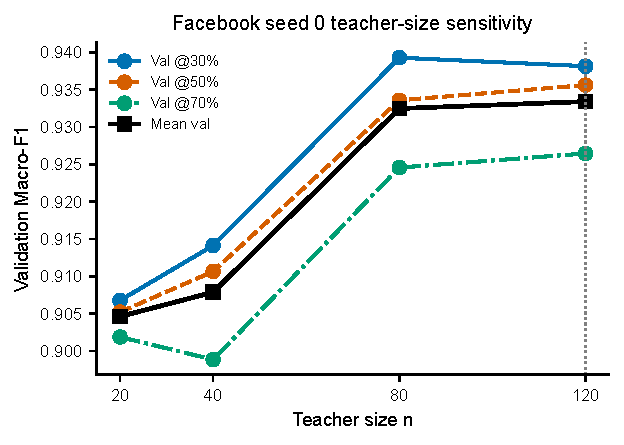
\includegraphics[width=0.72\linewidth]{figures/fig_s8_teacher_size.pdf}
\end{center}

\section{S9 Edge scorer and training losses}
GCN (2 layers, hidden 64, dropout 0.4); concatenation fusion in the core comparison; heteroscedastic decoder;
$\mathcal{L}=0.5\,\mathcal{L}_{\mathrm{CE}}+1.0\,\mathcal{L}_{\mathrm{NLL}}+0.2\,\mathcal{L}_{\mathrm{hinge}}$
with ranking margin $0.1$ and $256$ sampled pairs.
Gated and cross-attention fusions are ablations only.

\section{S10 Uncertainty estimation}
$\sigma_e=\exp(\tfrac12\log\sigma_e^2)$ via Gaussian NLL with variance floor $10^{-6}$ and $\log\sigma^2$ clamped to $[-8,4]$.
Pruning does \textbf{not} use $\sigma_e$; ranking uses $\mu_e$ only.

\section{S11 Exact-budget pruning}
\begin{algorithm}[H]
\caption{Unconstrained exact-budget prune (reported comparison)}
\begin{algorithmic}[1]
\Require importance $\mu$, removal rate $r$, undirected edge count $m$
\State $n_{\mathrm{keep}}\leftarrow m-\mathrm{round}(r\cdot m)$
\State Keep the top $n_{\mathrm{keep}}$ edges by descending $\mu$
\end{algorithmic}
\end{algorithm}
Implementation uses \texttt{torch.argsort(importance, descending=True)} without \texttt{stable=True}.
Tie order among equal $\mu$ values is therefore implementation-dependent and is not claimed to be stable.
Constraint-aware mode exists in code but is disabled in the reported multi-seed comparison.

\section{S12 Baseline implementation details}
All baselines are converted to the same exact-budget prune: keep the top $(1-r)|E|$ undirected edges by descending score via \texttt{budget\_prune\_unconstrained}.
They are simplified reimplementations adapted to this protocol, not bit-for-bit reproductions of the original publications.

\paragraph{Random.}
Uniform random scores in $[0,1]$ with seed-controlled RNG; higher score kept.
No training.

\paragraph{ILP-GCN.}
Two-layer GCN encoder (hidden $64$) with MLP link scorer trained by positive/negative edge BCE for \texttt{ilp\_epochs} (LastFM/Facebook/GitHub: $25/20/15$).
Importance follows the parent ILP form $W_{\mathrm{ILP}}=\alpha/(S+\varepsilon)$ mixed with uniform initial weights ($\gamma{=}0.5$); higher $W$ is retained.
Code: \path{src/sparsification/original_ilp.py}.

\paragraph{NeuralSparse.}
Simplified task-driven scorer: one GCN layer + MLP edge head; joint Adam training with node-classification CE on the train mask minus $0.01\times\mathrm{mean}(\mathrm{score})$ for \texttt{ilp\_epochs} epochs (same schedule as ILP-GCN in the grid).
After training, sigmoid edge scores are pruned under the exact budget.
This is not the full NeuralSparse $k$-neighbor sampler from Zheng et al.; it is a matched-budget adaptation.
Code: \path{src/sparsification/baselines/neuralsparse.py}.

\paragraph{PTDNet.}
Simplified topological-denoising scorer: two GCN layers + MLP denoise head; loss $=$ train-mask CE $+\,0.1\times\mathrm{mean}(\mathrm{score})$ for \texttt{ilp\_epochs} epochs.
Sigmoid scores are pruned under the exact budget.
Not a full reproduction of Luo et al.'s PTDNet; matched-budget adaptation.
Code: \path{src/sparsification/baselines/ptdnet.py}.

\paragraph{Resistance proxy.}
Effective-resistance-inspired ranking (degree-based / structural proxy path in \texttt{effective\_resistance\_proxy}).
It is not an independent reproduction of DSpar.
Duplicate records from the same resistance-based implementation were removed before aggregation ($n{=}10$ seeds).

\section{S13 Hyperparameters and training stages}
Four distinct training stages appear in the CILP pipeline (plus downstream evaluation):
\begin{center}\small
\begin{tabular}{@{}p{3.0cm}p{4.2cm}p{5.4cm}@{}}
\toprule
Stage & Epochs (LF/FB/GH) & Role \\
\midrule
Teacher encoder pretrain & $25/25/15$ & Frozen encoder/classifier for counterfactual probes \\
Surrogate MLP fit & $60/60/60$ & Fit \texttt{SurrogateEdgeImportance} on sampled teacher labels; expands targets to all edges for NLL; also yields S19 metrics \\
CILP scorer train & $25/25/15$ & End-to-end \texttt{CAILPSocial}; pruning uses its $\mu_e$ \\
Downstream GCN eval & $50/40/35$ & Fresh GCN on $G_r$ after pruning \\
ILP/NS/PTDNet train & $25/20/15$ & Baseline scorer epochs (not used by CILP) \\
\bottomrule
\end{tabular}
\end{center}
``Surrogate epochs'' and ``scorer epochs'' are therefore different models: the $60$-epoch surrogate is not the ranking scorer.
\begin{center}\scriptsize
\begin{longtable}{@{}p{2.2cm}p{4.2cm}p{6.8cm}@{}}
\caption{Hyperparameters used in the reported multi-seed comparison.}\\
\toprule Group & Parameter & Value \\ \midrule \endfirsthead
\toprule Group & Parameter & Value \\ \midrule \endhead
Model & encoder\_type & gcn \\
Model & num\_layers & 2 \\
Model & hidden\_dim & 64 \\
Model & dropout (CILP) & 0.4 \\
Model & fusion (core) & concat \\
Model & decoder & ImportanceDecoder hidden 64, dropout 0.2, ReLU \\
Model & mu activation & sigmoid \\
Model & logvar clamp & [-8, 4] \\
Model & LayerNorm in fusion & yes (ConcatFusion) \\
Model & NodeEncoder residual/norm defaults & residual=True, norm=True \\
Optimization & optimizer (CILP) & Adam \\
Optimization & learning\_rate (CILP) & 1e-3 \\
Optimization & weight\_decay (CILP) & Not explicitly configured; library default used (0.0) \\
Optimization & scheduler & Not explicitly configured; none used \\
Optimization & teacher\_encoder\_lr & 1e-2 \\
Optimization & surrogate\_mlp\_epochs & 60 (SurrogateEdgeImportance; not the CILP ranking scorer) \\
Optimization & surrogate\_hidden & 64 \\
Optimization & early\_stopping\_patience & Not explicitly configured; fixed epoch loops \\
Optimization & batch\_size & Not explicitly configured; full-batch graphs \\
Optimization & gradient\_clipping & Not explicitly configured; none used \\
Optimization & downstream\_classifier & 2-layer GCN, hidden 64, dropout 0.5 \\
Optimization & downstream\_lr & 1e-2 \\
Optimization & downstream\_weight\_decay & 5e-4 \\
Loss & lambda\_CE & 0.5 \\
Loss & lambda\_NLL & 1.0 \\
Loss & lambda\_rank & 0.2 \\
Loss & ranking\_margin & 0.1 \\
Loss & ranking\_num\_pairs & 256 \\
Loss & NLL variance floor & 1e-6 \\
Teacher & teacher\_n LastFM & 50 \\
Teacher & teacher\_n Facebook & 120 \\
Teacher & teacher\_n GitHub & 40 \\
Teacher & teacher\_epochs (encoder pretrain) LF/FB/GH & 25/25/15 \\
Teacher & surrogate\_mlp\_epochs (all datasets) & 60 \\
Teacher & cailp\_scorer\_epochs LF/FB/GH & 25/25/15 \\
Teacher & downstream\_epochs LastFM/Facebook/GitHub & 50/40/35 \\
Teacher & baseline\_scorer\_epochs (ILP/NS/PTD) LF/FB/GH & 25/20/15 \\
Teacher & sampling & stratified\_edge\_sample (degree$\times$cosine quartiles) \\
Teacher & beta & (1.0,0.5,1.0,0.3,0.5,0.5) \\
Teacher & beta tuned? & No; fixed across datasets \\
Teacher & zero-range handling & hi-lo<1e-12 → zeros \\
Pruning & rule & keep top (1-r)|E| by descending mu \\
Pruning & rounding & n\_keep = m - int(round(r*m)) \\
Pruning & ties & torch.argsort without stable=True; order not guaranteed \\
Pruning & constraints & Disabled in reported multi-seed comparison \\
Statistics & CI & mean ± t\_0.975,n-1 × SEM (paired t sampling dist.) \\
Statistics & hypothesis tests & two-sided Wilcoxon on paired diffs (primary) \\
Statistics & Holm family (i) & Within dataset: 4 CILP vs Task-only metrics \\
Statistics & Holm family (ii) & Within dataset: CILP vs baseline AUC contrasts \\
Statistics & effect size & dz = mean(diff)/sd(diff) \\
\bottomrule
\end{longtable}
\end{center}


\section{S14 Complete per-budget results}
\begin{center}\scriptsize
\begin{tabular}{@{}llccccccccc@{}}
\toprule
Dataset & Method & 0.1 & 0.2 & 0.3 & 0.4 & 0.5 & 0.6 & 0.7 & 0.8 & 0.9 \\
\midrule
LastFM & CILP & 0.792$\pm$0.019 & 0.792$\pm$0.024 & 0.786$\pm$0.040 & 0.761$\pm$0.052 & 0.769$\pm$0.061 & 0.743$\pm$0.070 & 0.715$\pm$0.071 & 0.671$\pm$0.067 & 0.590$\pm$0.059 \\
 & Task-only & 0.777$\pm$0.031 & 0.765$\pm$0.040 & 0.758$\pm$0.062 & 0.736$\pm$0.071 & 0.730$\pm$0.083 & 0.704$\pm$0.080 & 0.673$\pm$0.081 & 0.623$\pm$0.077 & 0.567$\pm$0.066 \\
 & ILP-GCN & 0.796$\pm$0.022 & 0.783$\pm$0.057 & 0.801$\pm$0.019 & 0.792$\pm$0.016 & 0.776$\pm$0.023 & 0.725$\pm$0.041 & 0.702$\pm$0.032 & 0.637$\pm$0.030 & 0.570$\pm$0.035 \\
 & PTDNet & 0.791$\pm$0.024 & 0.788$\pm$0.025 & 0.795$\pm$0.025 & 0.789$\pm$0.019 & 0.788$\pm$0.013 & 0.776$\pm$0.017 & 0.760$\pm$0.018 & 0.733$\pm$0.019 & 0.670$\pm$0.037 \\
 & NeuralSparse & 0.754$\pm$0.018 & 0.708$\pm$0.026 & 0.665$\pm$0.022 & 0.637$\pm$0.013 & 0.602$\pm$0.013 & 0.563$\pm$0.025 & 0.551$\pm$0.021 & 0.534$\pm$0.019 & 0.505$\pm$0.027 \\
 & Random & 0.797$\pm$0.029 & 0.782$\pm$0.028 & 0.773$\pm$0.016 & 0.759$\pm$0.024 & 0.745$\pm$0.036 & 0.702$\pm$0.035 & 0.696$\pm$0.036 & 0.653$\pm$0.026 & 0.583$\pm$0.021 \\
 & Resistance proxy & 0.741$\pm$0.024 & 0.658$\pm$0.037 & 0.613$\pm$0.031 & 0.590$\pm$0.027 & 0.558$\pm$0.027 & 0.530$\pm$0.026 & 0.524$\pm$0.020 & 0.497$\pm$0.014 & 0.480$\pm$0.009 \\
\midrule
Facebook & CILP & 0.932$\pm$0.011 & 0.931$\pm$0.012 & 0.931$\pm$0.012 & 0.929$\pm$0.012 & 0.927$\pm$0.013 & 0.924$\pm$0.014 & 0.919$\pm$0.014 & 0.912$\pm$0.014 & 0.905$\pm$0.012 \\
 & Task-only & 0.919$\pm$0.016 & 0.914$\pm$0.019 & 0.909$\pm$0.022 & 0.907$\pm$0.022 & 0.905$\pm$0.022 & 0.903$\pm$0.020 & 0.902$\pm$0.018 & 0.900$\pm$0.015 & 0.898$\pm$0.012 \\
 & ILP-GCN & 0.939$\pm$0.004 & 0.939$\pm$0.004 & 0.938$\pm$0.004 & 0.936$\pm$0.004 & 0.933$\pm$0.002 & 0.927$\pm$0.005 & 0.920$\pm$0.006 & 0.909$\pm$0.003 & 0.897$\pm$0.006 \\
 & PTDNet & 0.939$\pm$0.005 & 0.936$\pm$0.005 & 0.931$\pm$0.005 & 0.926$\pm$0.007 & 0.921$\pm$0.007 & 0.915$\pm$0.007 & 0.911$\pm$0.006 & 0.906$\pm$0.007 & 0.902$\pm$0.006 \\
 & NeuralSparse & 0.929$\pm$0.005 & 0.924$\pm$0.004 & 0.917$\pm$0.005 & 0.906$\pm$0.003 & 0.898$\pm$0.005 & 0.891$\pm$0.006 & 0.888$\pm$0.006 & 0.884$\pm$0.005 & 0.884$\pm$0.007 \\
 & Random & 0.935$\pm$0.005 & 0.932$\pm$0.005 & 0.928$\pm$0.005 & 0.922$\pm$0.006 & 0.917$\pm$0.006 & 0.911$\pm$0.006 & 0.903$\pm$0.006 & 0.897$\pm$0.005 & 0.891$\pm$0.004 \\
 & Resistance proxy & 0.899$\pm$0.005 & 0.889$\pm$0.005 & 0.888$\pm$0.006 & 0.888$\pm$0.006 & 0.886$\pm$0.007 & 0.886$\pm$0.006 & 0.888$\pm$0.007 & 0.889$\pm$0.007 & 0.891$\pm$0.006 \\
\midrule
GitHub & CILP & 0.814$\pm$0.006 & 0.813$\pm$0.006 & 0.812$\pm$0.005 & 0.811$\pm$0.005 & 0.809$\pm$0.006 & 0.809$\pm$0.006 & 0.809$\pm$0.005 & 0.806$\pm$0.004 & 0.803$\pm$0.004 \\
 & Task-only & 0.811$\pm$0.007 & 0.809$\pm$0.006 & 0.807$\pm$0.008 & 0.808$\pm$0.007 & 0.806$\pm$0.007 & 0.806$\pm$0.006 & 0.804$\pm$0.005 & 0.803$\pm$0.006 & 0.801$\pm$0.007 \\
 & ILP-GCN & 0.816$\pm$0.007 & 0.818$\pm$0.005 & 0.816$\pm$0.005 & 0.815$\pm$0.004 & 0.813$\pm$0.005 & 0.812$\pm$0.006 & 0.810$\pm$0.005 & 0.808$\pm$0.003 & 0.807$\pm$0.004 \\
 & PTDNet & 0.816$\pm$0.005 & 0.818$\pm$0.004 & 0.817$\pm$0.005 & 0.815$\pm$0.006 & 0.813$\pm$0.004 & 0.812$\pm$0.005 & 0.809$\pm$0.004 & 0.807$\pm$0.003 & 0.806$\pm$0.003 \\
 & NeuralSparse & 0.812$\pm$0.006 & 0.809$\pm$0.006 & 0.806$\pm$0.005 & 0.805$\pm$0.007 & 0.802$\pm$0.005 & 0.796$\pm$0.006 & 0.794$\pm$0.006 & 0.785$\pm$0.008 & 0.786$\pm$0.007 \\
 & Random & 0.814$\pm$0.004 & 0.813$\pm$0.005 & 0.811$\pm$0.006 & 0.810$\pm$0.006 & 0.807$\pm$0.005 & 0.807$\pm$0.004 & 0.804$\pm$0.005 & 0.806$\pm$0.004 & 0.806$\pm$0.004 \\
 & Resistance proxy & 0.806$\pm$0.007 & 0.806$\pm$0.006 & 0.806$\pm$0.005 & 0.808$\pm$0.005 & 0.807$\pm$0.005 & 0.808$\pm$0.004 & 0.808$\pm$0.004 & 0.808$\pm$0.005 & 0.808$\pm$0.005 \\
\bottomrule
\end{tabular}
\end{center}


\section{S15 Full per-seed results}
Machine-readable: \texttt{results/processed/authoritative\_results.csv}
($1{,}890$ rows; unique key dataset$\times$method$\times$seed$\times$edge\_removal\_rate).
The Stage~A freeze archive and checksums are recorded in \texttt{docs/stage\_a\_freeze\_manifest.md}.

\section{S16--S18 Paired statistical comparisons}
Hypothesis tests: two-sided Wilcoxon signed-rank on paired seed-wise differences (SciPy \texttt{wilcoxon}; \texttt{zero\_method='wilcox'}, \texttt{correction=False}, \texttt{method='auto'}).
Confidence intervals: mean difference $\pm t_{0.975,n-1}\mathrm{SEM}$ from the paired $t$ sampling distribution; paired $t$ $p$-values are computed in the analysis scripts but are not the primary reported tests.
Holm family~(ii) adjusts Wilcoxon $p$-values across CILP-versus-baseline AUC contrasts within each dataset.
\begin{center}\scriptsize
\begin{longtable}{@{}llrrrrrr@{}}
\caption{Paired contrasts (CILP minus comparator) on common seeds.}\\
\toprule
Dataset & Contrast & $n$ & $\Delta$ & 95\% CI & Wilcoxon $p$ & Holm $p$ & $d_z$ \\
\midrule
\endfirsthead
\toprule
Dataset & Contrast & $n$ & $\Delta$ & 95\% CI & Wilcoxon $p$ & Holm $p$ & $d_z$ \\
\midrule
\endhead
facebook & AUC vs Task-only & 10 & +0.0142 & [+0.0053,+0.0231] & 0.00390625 & 0.015625 & 1.137 \\
facebook & AUC vs ILP-GCN & 10 & -0.0029 & [-0.0091,+0.0033] & 0.625 & 1 & -0.333 \\
facebook & AUC vs PTDNet & 10 & +0.0026 & [-0.0052,+0.0104] & 0.625 & 1 & 0.235 \\
facebook & AUC vs NeuralSparse & 10 & +0.0177 & [+0.0113,+0.0241] & 0.00195312 & 0.011719 & 1.987 \\
facebook & AUC vs Random & 10 & +0.0069 & [+0.0006,+0.0131] & 0.0488281 & 0.14648 & 0.783 \\
facebook & AUC vs Resistance proxy & 10 & +0.0283 & [+0.0229,+0.0336] & 0.00195312 & 0.011719 & 3.786 \\
github & AUC vs Task-only & 10 & +0.0033 & [+0.0015,+0.0051] & 0.00195312 & 0.011719 & 1.292 \\
github & AUC vs ILP-GCN & 10 & -0.0024 & [-0.0040,-0.0008] & 0.00390625 & 0.015625 & -1.104 \\
github & AUC vs PTDNet & 10 & -0.0023 & [-0.0039,-0.0007] & 0.00585938 & 0.017578 & -1.029 \\
github & AUC vs NeuralSparse & 10 & +0.0084 & [+0.0062,+0.0106] & 0.00195312 & 0.011719 & 2.707 \\
github & AUC vs Random & 10 & +0.0010 & [+0.0001,+0.0019] & 0.105469 & 0.10547 & 0.800 \\
github & AUC vs Resistance proxy & 10 & +0.0022 & [+0.0002,+0.0042] & 0.0371094 & 0.074219 & 0.805 \\
lastfm & AUC vs Task-only & 10 & +0.0265 & [+0.0022,+0.0508] & 0.00390625 & 0.015625 & 0.781 \\
lastfm & AUC vs ILP-GCN & 10 & +0.0029 & [-0.0292,+0.0350] & 0.431641 & 0.55078 & 0.065 \\
lastfm & AUC vs PTDNet & 10 & -0.0232 & [-0.0527,+0.0063] & 0.0644531 & 0.19336 & -0.563 \\
lastfm & AUC vs NeuralSparse & 10 & +0.1037 & [+0.0748,+0.1326] & 0.00195312 & 0.011719 & 2.567 \\
lastfm & AUC vs Random & 10 & +0.0128 & [-0.0160,+0.0416] & 0.275391 & 0.55078 & 0.318 \\
lastfm & AUC vs Resistance proxy & 10 & +0.1344 & [+0.1041,+0.1648] & 0.00195312 & 0.011719 & 3.171 \\
\bottomrule
\end{longtable}
\end{center}


\section{S19 Surrogate-quality metrics}
\begin{center}\scriptsize
\begin{tabular}{@{}llccccc@{}}
\toprule
Dataset & Method & $n$ & MAE & Spearman & Kendall & ECE \\
\midrule
lastfm & CILP & 10 & 0.076 & 0.775 & 0.632 & 0.077 \\
lastfm & Task-only & 10 & 0.115 & 0.318 & 0.225 & 0.147 \\
facebook & CILP & 10 & 0.106 & 0.651 & 0.525 & 0.097 \\
facebook & Task-only & 10 & 0.164 & 0.104 & 0.068 & 0.175 \\
github & CILP & 10 & 0.237 & 0.255 & 0.211 & 0.165 \\
github & Task-only & 10 & 0.217 & 0.046 & 0.036 & 0.165 \\
\bottomrule
\end{tabular}

\end{center}
\noindent On GitHub, CILP has higher Spearman/Kendall agreement while Task-only has lower raw MAE and ECE is essentially tied.
Because sparsification ranks edges for deletion, rank correlation is the primary surrogate diagnostic; absolute MAE can favour flat predictors that are poor rankers.
Top-$k$ overlap and normalized MAE relative to target scale are recommended extensions.

\section{S20 Ablation study}
LastFM ablations (seeds $0$--$4$) are grouped scientifically below.
Facebook ablations were incomplete at the time of analysis.
Adversarial variants were omitted after a negative pilot.

\begin{center}\scriptsize
\begin{tabular}{@{}p{2.1cm}p{2.4cm}p{2.0cm}p{1.6cm}p{1.4cm}p{1.2cm}p{1.6cm}@{}}
\toprule
Group & Scientific name & Teacher & Prior & Fusion & Seeds & Status \\
\midrule
Fusion & Concatenation & multi-criteria & none & concat & 0--4 & complete \\
Fusion & Gated fusion & multi-criteria & none & gated & 0--4 & complete \\
Fusion & Cross-attention & multi-criteria & none & cross-attn & 0--4 & complete \\
Node prior & No node prior & multi-criteria & none & concat & 0--4 & complete \\
Node prior & Analytical mass & multi-criteria & analytical & concat & 0--4 & complete \\
Node prior & Degree prior & multi-criteria & degree & concat & 0--4 & complete \\
Node prior & PageRank prior & multi-criteria & PageRank & concat & 0--4 & complete \\
Node prior & Black Hole-inspired & multi-criteria & Black Hole & concat & 0--4 & complete \\
Teacher & Multi-criteria & multi-criteria & none & concat & 0--4 & complete \\
Teacher & Task-only & task-only & none & concat & 0--4 & complete \\
Optional & Adversarial variants & --- & --- & --- & --- & rejected / skipped \\
Context & ILP-GCN & N/A & N/A & N/A & 0--4 & complete \\
\bottomrule
\end{tabular}
\end{center}

Budgets reported in ablation figures: $0.3$, $0.5$, $0.7$.
Repository identifiers for these variants appear only in S29.

\section{S21 Multi-criteria versus task-only supervision}
We tested whether combining multiple deletion-importance criteria improves edge ranking relative to task-only supervision under the same encoder, fusion, optimization, budgets, and paired seeds.
\textbf{Family~(i) definition:} for each dataset, four paired metrics (CILP $-$ Task-only) form one family:
(i) sparsity--Macro-F1 AUC;
(ii) giant-component ratio at $50\%$;
(iii) bridge retention at $50\%$;
(iv) minority-degree retention at $50\%$.
Holm adjustment is applied to Wilcoxon $p$-values within each dataset family~(i).
\textbf{Family~(ii):} within each dataset, CILP-versus-baseline AUC contrasts form a separate Holm family (Supplementary Information~S16--S18); adjusted $p$-values are not interchangeable with family~(i).
\textbf{Decision rule:} multi-criteria supervision is supported across datasets when at least two metrics are supported (positive $\Delta$, Holm $p{<}0.05$) on at least two datasets.
The analysis rule was fixed before completion and integration of the GitHub grid; we do not claim timestamped preregistration beyond the Stage~A freeze record.
On LastFM, Facebook, and GitHub the within-dataset criterion is met (4/4 metrics each); multi-criteria supervision therefore satisfies the fixed support criterion on all three datasets.
This support is relative to the matched Task-only teacher and does not imply that CILP outperforms all established sparsifiers.
\begin{center}\scriptsize
\begin{longtable}{@{}llrrrrrrrcc@{}}
\caption{Paired CILP versus Task-only tests (common seeds). Family: four metrics per dataset; Holm adjustment on Wilcoxon $p$.}\\
\toprule
Dataset & Metric & CILP & Task-only & $\Delta$ & 95\% CI & Wilcoxon $p$ & Holm $p$ & $d_z$ & W/T/L \\
\midrule
\endfirsthead
\toprule
Dataset & Metric & CILP & Task-only & $\Delta$ & 95\% CI & Wilcoxon $p$ & Holm $p$ & $d_z$ & W/T/L \\
\midrule
\endhead
lastfm & AUC & 0.593 & 0.566 & +0.0265 & [+0.0022,+0.0508] & 0.003906 & 0.007812 & 0.781 & 9/0/1 \\
lastfm & GC @50\% & 0.928 & 0.772 & +0.1564 & [+0.0165,+0.2962] & 0.001953 & 0.007812 & 0.800 & 10/0/0 \\
lastfm & Bridge @50\% & 0.904 & 0.681 & +0.2230 & [+0.0318,+0.4142] & 0.001953 & 0.007812 & 0.835 & 10/0/0 \\
lastfm & Min-deg @50\% & 0.891 & 0.673 & +0.2182 & [+0.0149,+0.4214] & 0.01151 & 0.01151 & 0.768 & 8/2/0 \\
facebook & AUC & 0.739 & 0.725 & +0.0142 & [+0.0053,+0.0231] & 0.003906 & 0.01562 & 1.137 & 9/0/1 \\
facebook & GC @50\% & 0.923 & 0.626 & +0.2971 & [+0.1321,+0.4622] & 0.007686 & 0.02306 & 1.288 & 9/1/0 \\
facebook & Bridge @50\% & 0.827 & 0.422 & +0.4053 & [+0.1938,+0.6169] & 0.007686 & 0.02306 & 1.371 & 9/1/0 \\
facebook & Min-deg @50\% & 0.650 & 0.493 & +0.1569 & [+0.0204,+0.2935] & 0.01367 & 0.02306 & 0.822 & 8/0/2 \\
github & AUC & 0.648 & 0.645 & +0.0033 & [+0.0015,+0.0051] & 0.001953 & 0.007812 & 1.292 & 10/0/0 \\
github & GC @50\% & 0.903 & 0.674 & +0.2284 & [+0.0717,+0.3851] & 0.001953 & 0.007812 & 1.043 & 10/0/0 \\
github & Bridge @50\% & 0.802 & 0.483 & +0.3195 & [+0.1305,+0.5085] & 0.001953 & 0.007812 & 1.209 & 10/0/0 \\
github & Min-deg @50\% & 0.565 & 0.452 & +0.1136 & [+0.0270,+0.2002] & 0.003906 & 0.007812 & 0.938 & 9/0/1 \\
\bottomrule
\end{longtable}
\end{center}


\section{S22 Structural and group metrics}
Means at $50\%$ removal appear below; multi-budget ($30/50/70\%$) giant-component and bridge values are also reported in the main manuscript.
\begin{center}\scriptsize
\begin{tabular}{@{}llccc@{}}
\toprule
Dataset & Method & Giant-component ratio & Bridge retention & Minority-degree retention \\
\midrule
lastfm & CILP & 0.928 & 0.904 & 0.891 \\
lastfm & Task-only & 0.772 & 0.681 & 0.673 \\
lastfm & ILP-GCN & 0.880 & 0.920 & 0.909 \\
lastfm & PTDNet & 0.822 & 0.759 & 0.914 \\
lastfm & Random & 0.784 & 0.501 & 0.500 \\
facebook & CILP & 0.923 & 0.827 & 0.650 \\
facebook & Task-only & 0.626 & 0.422 & 0.493 \\
facebook & ILP-GCN & 0.966 & 0.979 & 0.964 \\
facebook & PTDNet & 0.754 & 0.607 & 0.630 \\
facebook & Random & 0.863 & 0.502 & 0.500 \\
github & CILP & 0.903 & 0.802 & 0.565 \\
github & Task-only & 0.674 & 0.483 & 0.452 \\
github & ILP-GCN & 0.925 & 0.685 & 0.666 \\
github & PTDNet & 0.925 & 0.687 & 0.746 \\
github & Random & 0.873 & 0.500 & 0.499 \\
\bottomrule
\end{tabular}

\end{center}

\section{S23 Runtime}
\texttt{train\_seconds} includes teacher construction and scorer fitting for CILP and Task-only; these components were not separately logged, so dominance cannot be attributed to teacher construction alone.
\begin{center}\scriptsize
\begin{tabular}{@{}llccc@{}}
\toprule
Dataset & Method & $n$ & Train seconds & Prune seconds \\
\midrule
lastfm & Random & 10 & 0.01$\pm$0.01 & 0.193$\pm$0.138 \\
lastfm & ILP-GCN & 10 & 5.20$\pm$2.05 & 0.052$\pm$0.088 \\
lastfm & PTDNet & 10 & 2.57$\pm$0.72 & 0.190$\pm$0.174 \\
lastfm & NeuralSparse & 10 & 4.09$\pm$1.41 & 0.053$\pm$0.097 \\
lastfm & Task-only & 10 & 254.63$\pm$149.00 & 0.115$\pm$0.140 \\
lastfm & CILP & 10 & 198.40$\pm$89.25 & 0.158$\pm$0.140 \\
facebook & Random & 10 & 0.00$\pm$0.00 & 0.107$\pm$0.118 \\
facebook & ILP-GCN & 10 & 8.55$\pm$1.95 & 0.068$\pm$0.103 \\
facebook & PTDNet & 10 & 5.09$\pm$1.44 & 0.206$\pm$0.299 \\
facebook & NeuralSparse & 10 & 6.56$\pm$1.95 & 0.109$\pm$0.142 \\
facebook & Task-only & 10 & 1635.33$\pm$541.98 & 0.030$\pm$0.021 \\
facebook & CILP & 10 & 1436.51$\pm$421.38 & 0.050$\pm$0.073 \\
github & Random & 10 & 0.00$\pm$0.01 & 0.037$\pm$0.005 \\
github & ILP-GCN & 10 & 7.43$\pm$0.34 & 0.034$\pm$0.004 \\
github & PTDNet & 10 & 3.87$\pm$0.29 & 0.036$\pm$0.006 \\
github & NeuralSparse & 10 & 4.82$\pm$0.29 & 0.036$\pm$0.005 \\
github & Task-only & 10 & 504.15$\pm$93.94 & 0.034$\pm$0.003 \\
github & CILP & 10 & 503.97$\pm$85.02 & 0.034$\pm$0.002 \\
\bottomrule
\end{tabular}

\end{center}

\section{S24 Failure cases and rejected hypotheses}
Adversarial pilot (LastFM seed 0, $50\%$): Macro-F1 $\approx0.666$ vs core $\approx0.829$.
Facebook teacher $n{=}40$ underperformed the development-selected $n{=}120$ setting (S8).
Stage~A GitHub grid: no method failures across seeds $0$--$9$, seven methods, and budgets $0.1$--$0.9$.

\section{S25 Constraint shortfalls}
Reported comparison: constraints off; achieved removals match requested budgets exactly under unconstrained ranking.

\section{S26 Reproducibility checklist}
Processed authoritative CSV/JSON ($1{,}890$ rows); Stage~A freeze manifest with SHA-256 checksums; consistency validator; fixed splits for all three datasets; negative pilots retained; figure provenance notes.
Paths: \path{docs/stage_a_freeze_manifest.md}, \path{docs/figure_data_provenance.md}.

\section{S27 Software and hardware}
Reported multi-seed runs used CPU execution (\texttt{device=cpu} in experiment logs); MPS is disabled in the device helper because several PyG scatter operations are unsupported.
Exact CPU model, core counts, and RAM for the machines that produced every grid row are not stored as structured metadata in the repository and therefore cannot be uniquely recovered.
Environment specification files declare Python 3.10 (\texttt{environment.yml}, \texttt{Dockerfile}); analysis regeneration on the present workstation used Python 3.9.6 with:
PyTorch 2.4.0, PyTorch Geometric 2.6.1, NetworkX 3.2.1, NumPy 1.26.4, SciPy 1.13.1, scikit-learn 1.6.1, matplotlib 3.9.4.
No \texttt{pip freeze} lockfile is present; \texttt{requirements.txt} lists version floors only.
BLAS backend was not recorded in experiment logs.

\section{S28 Data and code availability details}
Public SNAP/MUSAE releases for LastFM, Facebook, and GitHub.
Processed graphs: \path{data/processed/}.
Fixed splits: \path{data/splits/}.
Authoritative store: \path{results/processed/authoritative_results.csv} ($1{,}890$ rows).
GitHub raw per-seed outputs: \path{results/raw/grid/}.
Stage~A freeze archive: \path{results/frozen/}.
Regenerated figures/tables: \path{paper/}.
Regeneration and consistency-check scripts: \path{scripts/}.
No DOI is claimed in this draft.

\section{S29 Repository ID mapping}
Internal experiment identifiers appear only in this table.
\begin{center}\scriptsize
\begin{longtable}{@{}llp{7.2cm}@{}}
\caption{Repository ID mapping (internal identifiers; not used elsewhere in the PDFs).}\\
\toprule
Repository ID & Scientific description & Notes \\
\midrule
\endfirsthead
\toprule
Repository ID & Scientific description & Notes \\
\midrule
\endhead
A1\_full\_core & CILP core configuration & Reported main method \\
A2\_original\_ilp & ILP-GCN parent baseline & Parent method \\
A8\_concat & Multi-criteria teacher with concatenation & Fusion-matched to task-only \\
A9\_gated & Multi-criteria teacher with gated fusion & Ablation \\
A10\_cross\_attn & Multi-criteria teacher with cross-attention & Ablation; not core \\
A19\_no\_mass & No node prior & Ablation \\
A20\_analytical\_mass & Analytical mass prior & Ablation \\
A23\_degree\_prior & Degree prior & Ablation \\
A24\_pagerank\_prior & PageRank prior & Ablation \\
A25\_no\_adversarial & No adversarial module & Equivalent to core path \\
A26\_repr\_disc & Representation discriminator & Skipped; rejected pilot \\
A27\_mask\_gan & Mask GAN & Skipped; rejected pilot \\
A28\_gan\_without\_ilp & GAN without ILP & Skipped; rejected pilot \\
A31\_single\_obj\_concat & Task-only counterfactual teacher & Matched ablation \\
A31\_single\_obj\_gated & Task-only with gated fusion & Ablation \\
A32\_black\_hole\_mass & Black Hole-inspired prior & Ablation \\
cailp\_multi & CILP main grid key & JSON method key \\
cailp\_a31 & Task-only grid key & JSON method key \\
\bottomrule
\end{longtable}
\end{center}


\bibliographystyle{plainnat}
\bibliography{references}
\end{document}
